\documentclass[10pt]{beamer}

\usetheme[progressbar=frametitle]{metropolis}
\usepackage{appendixnumberbeamer}
\usepackage{pgfpages}
\usepackage{booktabs}
\usepackage{xcolor}
\usepackage{mathtools}

\usepackage{pgfplots}

\usepgfplotslibrary{dateplot}

\setbeameroption{slides only}
%\setbeameroption{show only notes}
%\setbeameroption{show notes on second screen=right}
\usepackage{xspace}
\newcommand{\themename}{\textbf{\textsc{metropolis}}\xspace}

\title{Labor Markets and Technological Change: Evidence from Electronic Health Records}

\subtitle{Hanna Glenn\\ \small Advisor: Dr. Ian McCarthy}
 \date{\today}

\setbeamertemplate{caption}{\raggedright\insertcaption\par}
\setbeamertemplate{itemize item}{\scalebox{.6}{$\blacktriangleright$ }}     
\setbeamertemplate{itemize subitem}{\scalebox{.8}{$\centerdot$ }} 

\begin{document}

\maketitle

\setbeamercolor{background canvas}{bg=white}



\section[Motivation]{Motivation}

\begin{frame}{The Broad Question}
\begin{itemize}
    \item Longstanding topic in economics: relationship between technology and employment
    \vspace{2mm}
    \begin{itemize}
        \item Displacement?
        \item Productivity?
    \end{itemize}
    \vspace{3mm}
    \item Investigated in many settings
    \vspace{3mm}
    \item This paper: specific healthcare setting
\end{itemize}

\end{frame}

\begin{frame}[fragile]{What is an Electronic Health Record?}
``An electronic health record is the systematized collection of patient and population electronically stored health information in a digital format"

\vspace{3mm}

What it can do:
\begin{itemize}
    \item Paper $\rightarrow$ computerization
    \item Communication
    \item Decision making assistance
\end{itemize}

\end{frame}

\begin{frame}[fragile]{HIT: Great (Expected) Potential in Healthcare}
\begin{alertblock}{Cost Saving}
\begin{itemize}
    \item Possible cost reduction of hundreds of billions of dollars \\ \scriptsize (Hillestad et al 2005)
\end{itemize}
\end{alertblock}

\begin{alertblock}{Quality Improvement}
\begin{itemize}
    \item Improved efficiency, patient safety improvements, physicians have decision support that could prevent unnecessary complications, etc.
\end{itemize}
\end{alertblock}

\vspace{4mm}

Significant policy push for EHR implementation: HITECH Act, 2008 provided financial incentive for hospitals to implement EHRs
\begin{itemize}
    \item \textcolor{blue}{The percentage of hospitals with basic EHR capability rose from 9$\%$ in 2008 to 84$\%$ in 2015.} \scriptsize (Health IT Dashboard)
\end{itemize}

\end{frame}


\begin{frame}{Physician Response to EHRs}
\begin{center}
    
\includegraphics[scale=.3]{graphics/News Clip3.PNG}
    
    \vspace{3mm}
    
    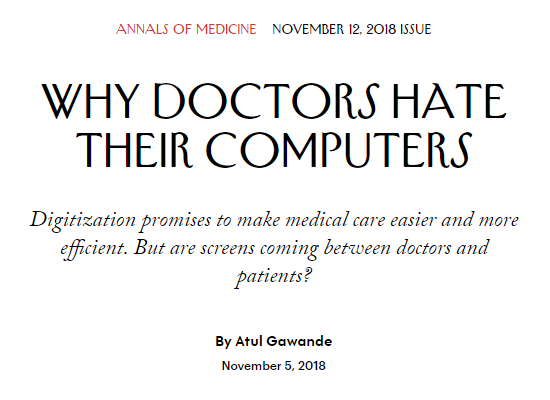
\includegraphics[scale=.3]{graphics/News Clip2.PNG}
\end{center}

\end{frame}


\begin{frame}{This Paper}

Did EHR implementation in hospitals affect physician labor market decisions?
\begin{itemize}
    \item Intensive Margin / Productivity
    \item Extensive Margin / Retirement
    \item Hospital $\rightarrow$ Office
\end{itemize}

\end{frame}


\section{Contribution}

\begin{frame}{Literature}
\small
\begin{columns}
\setlength{\tabcolsep}{-5pt}
    \column{0.4\textwidth}
        \centering
        \underline{ Technology $\rightarrow$ Labor }
        \vspace{-1mm}
        \begin{itemize}
            \item Erosion effect vs. wage effect \\ \vspace{1mm}
            \tiny (Zeira $\&$ Joseph 2011, EJ)
            
            \footnotesize
            
            \item Cause retirement? \\ \vspace{1mm}
            \tiny (Schleife 2006, Labour; Cavapozzi et al 2013, AE; Roger et al 2006, EJ; Friedburg 2003, ILRR)
            
            \footnotesize
            
            \item Older, well educated members of labor force exited at higher rates due to computerization \\ \vspace{1mm}
            \tiny (Willis and Hudomiet 2021, Labour)
        \end{itemize}
        
        
        \column{0.4\textwidth}
        \centering
        
        \pause
        
        \color{blue}
        \underline{ Contribution }
        
        \vspace{1mm}
 
            \begin{itemize}
            \color{blue}
                \item Healthcare spending is extremely high
                \item Population of physicians - possible shortages / access to care issues
            \end{itemize}

        
\end{columns}
\end{frame}



\begin{frame}{Literature}
\small
\begin{columns}
\setlength{\tabcolsep}{-5pt}
        \column{0.4\textwidth}
        \centering
        \underline{ EHR $\rightarrow$ Healthcare }
        \vspace{-1mm}
        \begin{itemize}
            \item Small improvements for severe health conditions \\ \vspace{1mm}
            \tiny(Agha 2014, JHE; McCullough et al 2016, RAND)
            
            \footnotesize
            
            \item No decrease in cost \\ \vspace{1mm}
            \tiny (Agha 2014, JHE; Dranove et al 2019, AEJ) 
            
            \footnotesize
            
            \item Productivity and opinion about EHRs varies drastically \\ \vspace{1mm}
            \tiny (Hitt $\&$ Tambe 2016, ILRR; Butler $\&$ Johnson 2016, IJHEM; Meyerhoefer et al 2016, ILRR)
        \end{itemize}
        
        \pause
        
        \column{0.4\textwidth}
        \centering
        \color{blue}
        \underline{ Contribution }
        \vspace{1mm}
        \begin{itemize}
        \color{blue}
            \item No empirical work on EHR/physician effects
            \item Speaks to the puzzling results
            \item Time period 
        \end{itemize}
        
        
\end{columns}

\end{frame}




\section{Data}

\begin{frame}{Data}
    \underline{Main: CMS Shared Patient Data (2009-2015)}
    \begin{itemize}
        \item Hospital-physician pairs: bill for same patient under Medicare
        \item Physician (PCP, hospitalist, internist) works in the hospital
    \end{itemize}
    
    \vspace{3mm}
    
    \underline{EHR Use:}
    \begin{itemize}
        \item AHA Survey
    \end{itemize}
    
    \vspace{3mm}
    
    \underline{Other:}
    \begin{itemize}
        \item Physician Compare
    \end{itemize}
    
    \vspace{3mm}
    
    Aggregated to physician level
\end{frame}


\begin{frame}{Variables}
Labor Market Outcomes:
\begin{itemize}
\item Productivity:
\begin{itemize}
    \item Patients visited in hospitals
\end{itemize}
\end{itemize}
\begin{itemize}
\item \color{gray} Retirement
\end{itemize}
\begin{itemize}
\item \color{gray} Work Setting:
\begin{itemize}
    \item \color{gray} Maintaining billable activity only outside of hospitals
    \item \color{gray} Level of billable activity outside of hospitals
\end{itemize}
\end{itemize}

EHR Use:
\vspace{-2mm}
\begin{itemize}
    \item Indicator for any exposure to EHR
    \item \color{gray} Fraction of hospitals exposed to EHR
\end{itemize}

Other:
\vspace{-2mm}
\begin{itemize}
    \item Years of experience
    \item Hospital characteristics
\end{itemize}

\end{frame}


\begin{frame}{Data}
    \centering
    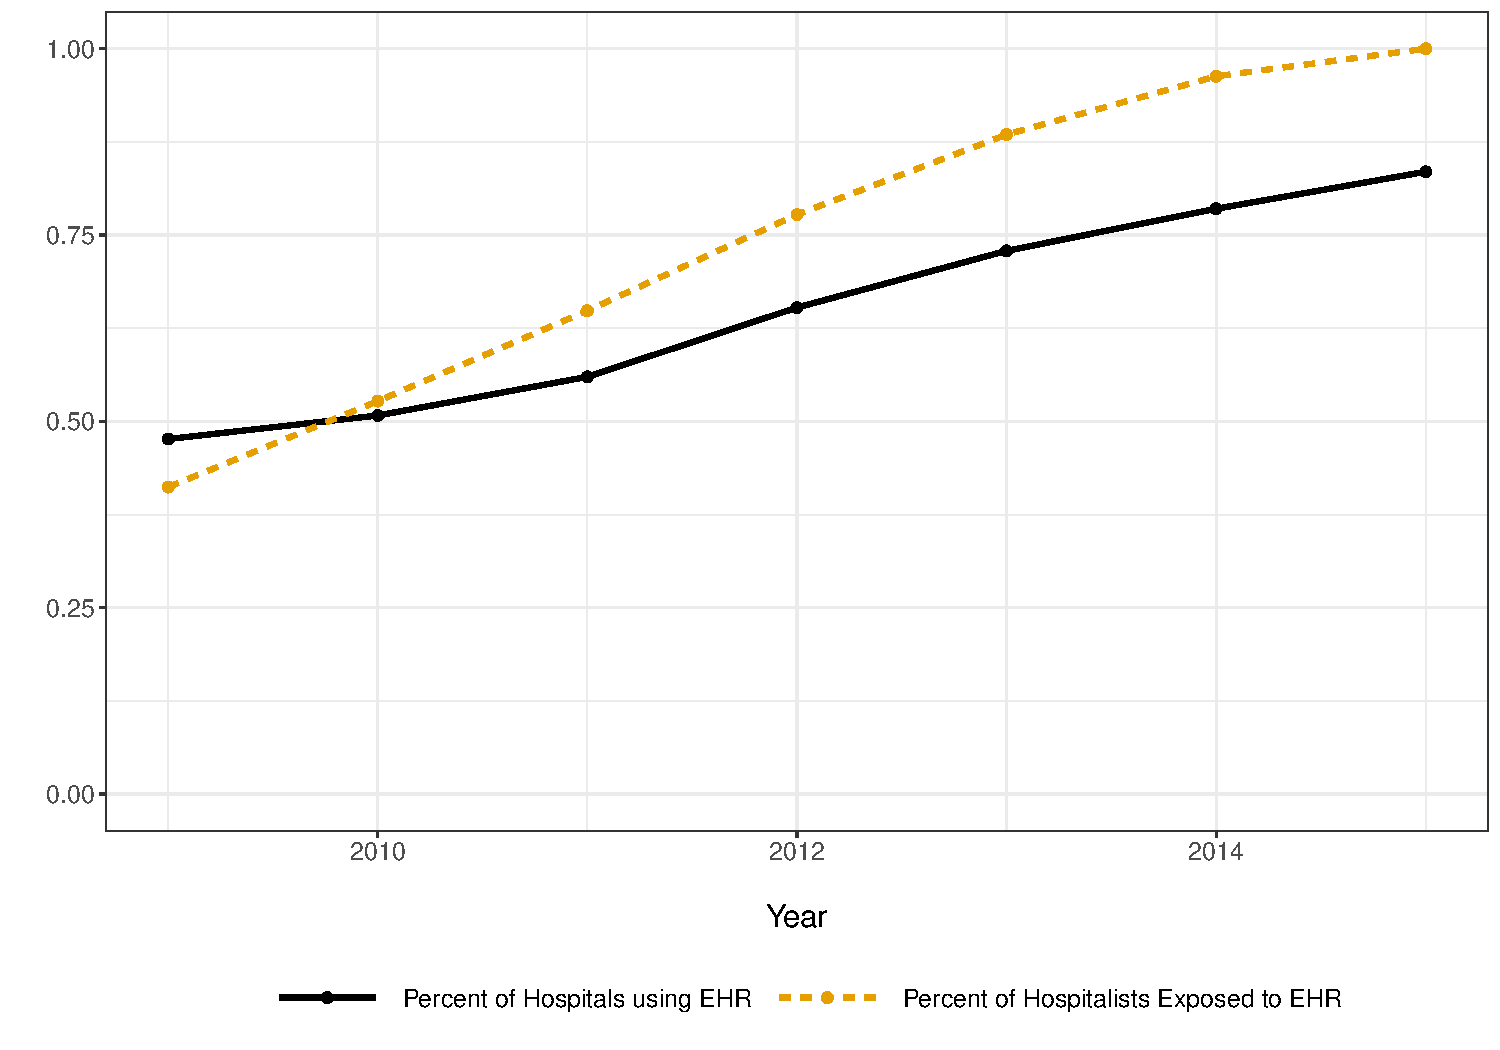
\includegraphics[scale=.5]{Objects/sum_stats_year.pdf}
\end{frame}

\begin{frame}{Data}
\centering
    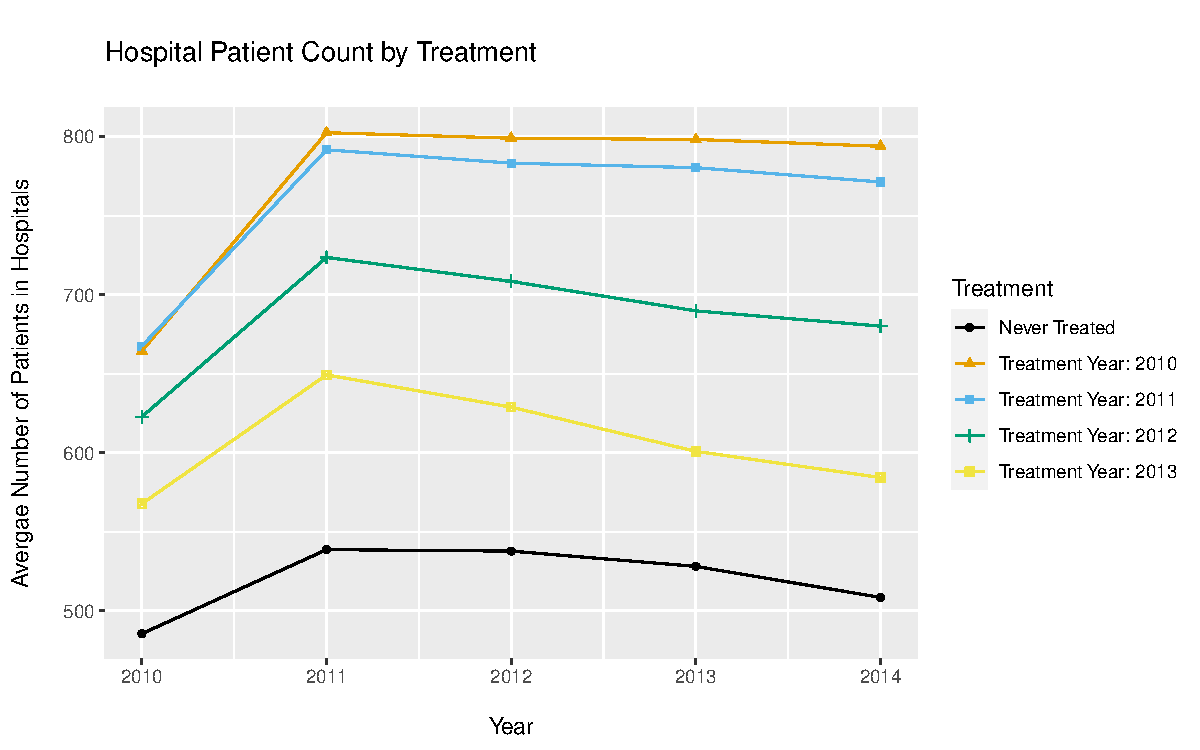
\includegraphics[scale=.5]{Objects/cont_treatment_graph.pdf}
    
\end{frame}


\section{Analysis}


\begin{frame}{Event Study}
\begin{equation*}
    y_{it}=\alpha_i+\delta_t+q_{it}'\lambda+\sum_{k=-4}^4 \beta_kz_{i,t-k} + \varepsilon_{it}
\end{equation*}

\vspace{4mm}

\begin{align*}
    y_{it} &: \text{Outcomes} \hspace{30mm}\\
    \alpha_i, \delta_t &: \text{Fixed Effects}\hspace{30mm}\\
    q_{it} &: \text{Physician/hospital characteristics}\hspace{30mm}\\
    z_{i,t-k} &: \text{Exposure to EHR} \hspace{30mm}
\end{align*}

    
\end{frame}

\section{Results}


\begin{frame}{Dep. Variable: Patients Billed with Hospitals}
\begin{figure}[ht]
        \begin{minipage}[b]{0.47\linewidth}
            \centering
            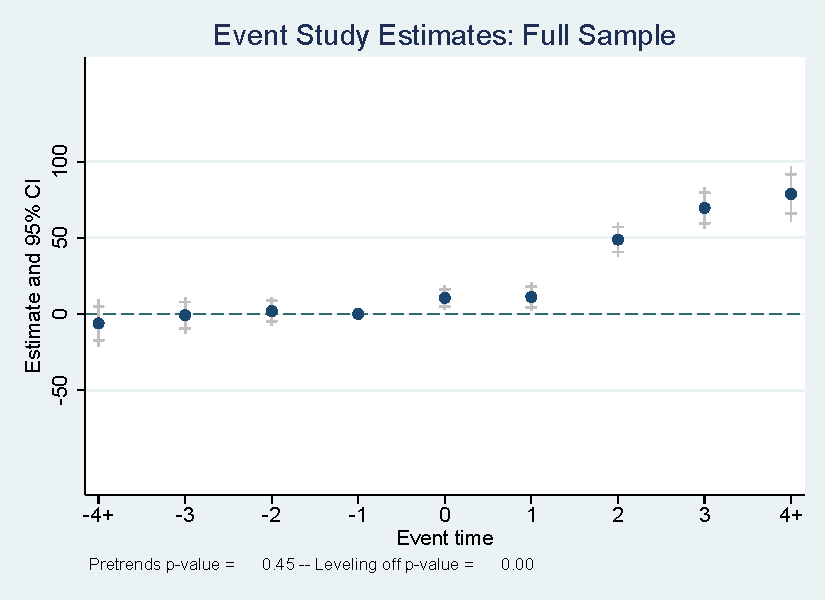
\includegraphics[width=\textwidth]{Objects/xtevent_fullsample.pdf}
        \end{minipage}
        \hspace{0.2cm}
        \begin{minipage}[b]{0.47\linewidth}
            \centering
            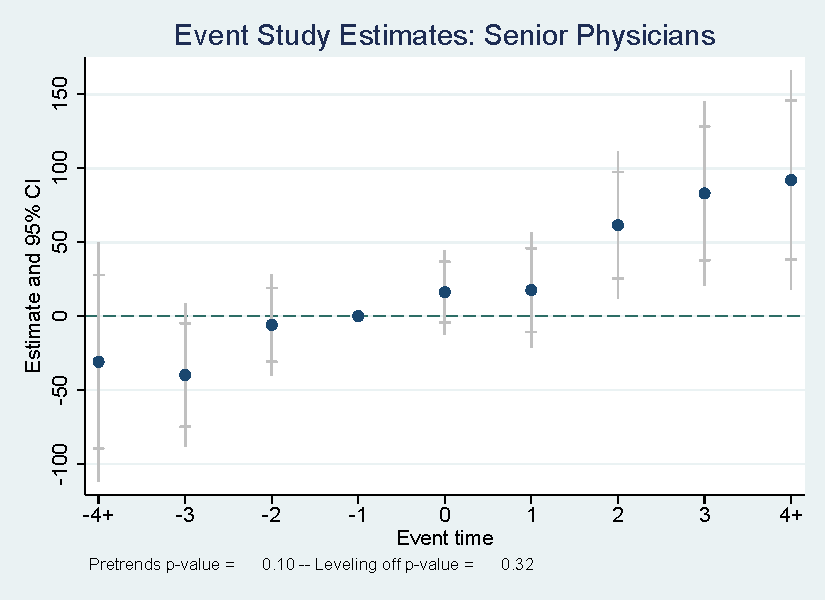
\includegraphics[width=\textwidth]{Objects/xtevent_oldsample.pdf}
        \end{minipage}
    \end{figure}
\end{frame}

\begin{frame}{Summary}
\begin{itemize}
    \item Despite physician response to EHRs, those who stick around do become more productive
    \vspace{3mm}
    
    \item Complementary relationship between physicians and EHRs
    \vspace{3mm}
    
    \item Older physicians see (slightly) greater productivity increases 
    \vspace{3mm}
    
\end{itemize}
\end{frame}







\section{Continuing Work}

\begin{frame}{Plans for this paper}
    \begin{itemize}
        \item Analysis on retirement decision of physicians: requires a better understanding of why physicians would drop out of this Medicare data
        \item See if there are any specific years driving these results
        \item Endogenous treatment? (Bandwidth, state privacy laws as IV)
    \end{itemize}
\end{frame}

\begin{frame}[plain]{}
\centering
    Thank you!
\end{frame}



\end{document}
